\section{Structural Hazards}

\subsection{Detection}
The structural hazard occurs in data memory and register file.

\subsection{Handling}
The structural hazard in data memory is solved by using 2 memory units, one for instructions and one for data. Both have the same specs \emph{(previously mentioned)}.

However, structural hazard in register file is handled by forcing the write back to happen in the first half of the clock cycle and register reading from decode and fetch to happen in the second half.

\section{Data Hazards}

Figure \ref{fig:hdu} shows the hazard detection unit.
\begin{figure}[hp]
    \centering
    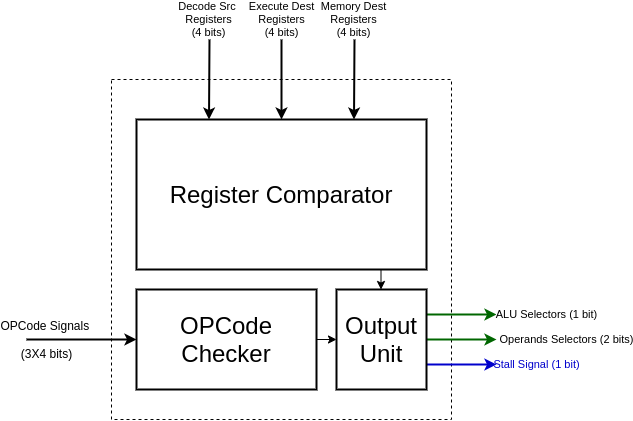
\includegraphics[width=0.8\textwidth]{images/hdu}
    \caption{Hazard Detection Unit Diagram}
    \label{fig:hdu}
\end{figure}

\subsection{Detection}

\subsubsection{Hazard Detection Unit (HDU)}

HDU consists of 3 parts:
\begin{itemize}
    \item \textbf{OPCode Checker:} checks the opcode of the current instruction to check whether it will cause data hazard or not. Also, it checks for \emph{load-use case}, in order to activate the stall signal.
    \item \textbf{Register Comparator:} compares the decode source registers with the destination registers of the execute and memory stages. Also, it compares the execute source registers with the destination registers of the memory stage.
    \item \textbf{Output Unit:} outputs stall signal in case of load and pop instructions (considering the branch special case). Also, it outputs ALU and decode operands selectors. 
\end{itemize}

\subsection{Handling}

\subsubsection{Stall}
Occurs only at Fetch and Decode stage, due to load(pop) use case.
\begin{itemize}
    \item Fetch same instruction (don't increment the program counter).
    \item Latch IF/ID buffer with the same values.
    \item Freeze Decode stage.
    \item Clear ID/EX buffer.
\end{itemize}

\subsubsection{Data Forwarding}
\begin{itemize}
    \item EX/MEM buffer $->$ Execute / Decode.
    \item ID/EX buffer $->$ Decode.
\end{itemize}

\section{Control Hazards}

\subsection{Detection}
The branch address calculation occurs in the Decode stage. So, the hazard might affect only the Fetch stage, which will be flushed in case of wrong address prediction.

\subsection{Handling}
\begin{itemize}
    \item At Fetch stage, always check the branch predictor and calculate the next address accordingly.
    \item At Decode stage, we have a \emph{Branch Address Unit} that checks whether the OPCode is of a branch operation. If so, it passes the address to the program counter and compares the correct address with the address of the counter to decide whether to flush the Fetch stage or not. 
\end{itemize}

\subsubsection{Flush}
Occurs only at Fetch Stage, due to wrong branch prediction at Decode stage.
\begin{itemize}
    \item Load new address in the program counter.
    \item Remove fetched instructions from IF/ID buffer.
\end{itemize}

\subsubsection{Dynamic Branch Prediction}
We use 2-bit branch predictor, which is a hash table of \emph{Finite State Machines} (FSMs) to predict whether the branch will be taken (1) or not (0) at each individual branch address.